\documentclass{standalone}
\usepackage{tikz} 
\usetikzlibrary{shapes}
% modular arithmetics etc. inspired by
%http://www.texample.net/tikz/examples/arithmetic-of-the-clock/
%TODO see also
%https://tex.stackexchange.com/a/66329
%https://tex.stackexchange.com/a/362672
\definecolor{hexcol0}{cmyk}{1,0,0,0} % cyan
\definecolor{hexcol1}{cmyk}{0,1,0,0}
\definecolor{hexcol2}{cmyk}{0,0,1,0}
\begin{document}
\newcounter{hexcellkind}
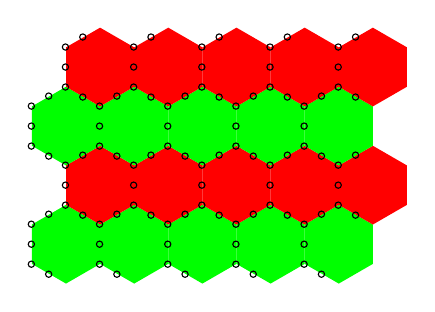
\begin{tikzpicture} 
  [  
     hexa/.style={shape=regular polygon, 
                  regular polygon sides=6, 
                  minimum size=1cm, 
		  rotate=30,
                  %draw,
                  anchor=south}, 
     tria/.style={shape=regular polygon, 
                  regular polygon sides=3, 
                  minimum size=.25cm, 
                  %%draw,
                  anchor=center},
     circ/.style={draw,
                  circle,
                  inner sep=2pt,
                  fill}
  ]
    \begin{scope}
        %\clip(0,0) rectangle (2,2);
        \foreach \j in {0,...,3}{% 
         \ifodd\j 
             \foreach \i in {0,...,4}{
		     	\node[hexa,red,fill=red] (h\j;\i) at ({(\i+1/2)*sin(60)},{\j/2+\j/4}) {};
	     }
        \else
	     \foreach \i in {0,...,4}{
		     \node[hexa,fill=green] (h\j;\i) at ({\i*sin(60)},{\j/2+\j/4}) {};
	    }
        \fi
	}
        \foreach \j in {0,...,3}{% 
             \foreach \i in {0,...,4}{
			  \path 
				  (h\j;\i.side 1) node[circle,draw,inner sep=0.8pt] (t1) {}
				  (h\j;\i.corner 2) node[circle,draw,inner sep=0.8pt] (t2) {}
				  (h\j;\i.side 2) node[circle,draw,inner sep=0.8pt] (t3) {}
				  (h\j;\i.corner 3) node[circle,draw,inner sep=0.8pt] (t4) {}
				  (h\j;\i.side 3) node[circle,draw,inner sep=0.8pt] (t5) {};
			  %\draw (t1) -- (t2) -- (t3) -- (t4) -- (t5) -- (t1);
	    }
        }
    \end{scope}

\end{tikzpicture}
\end{document}
